\documentclass[]{article}
\usepackage{lmodern}
\usepackage{amssymb,amsmath}
\usepackage{ifxetex,ifluatex}
\usepackage{fixltx2e} % provides \textsubscript
\ifnum 0\ifxetex 1\fi\ifluatex 1\fi=0 % if pdftex
  \usepackage[T1]{fontenc}
  \usepackage[utf8]{inputenc}
\else % if luatex or xelatex
  \ifxetex
    \usepackage{mathspec}
  \else
    \usepackage{fontspec}
  \fi
  \defaultfontfeatures{Ligatures=TeX,Scale=MatchLowercase}
\fi
% use upquote if available, for straight quotes in verbatim environments
\IfFileExists{upquote.sty}{\usepackage{upquote}}{}
% use microtype if available
\IfFileExists{microtype.sty}{%
\usepackage{microtype}
\UseMicrotypeSet[protrusion]{basicmath} % disable protrusion for tt fonts
}{}
\usepackage[margin=1in]{geometry}
\usepackage{hyperref}
\hypersetup{unicode=true,
            pdftitle={Assignment 3},
            pdfborder={0 0 0},
            breaklinks=true}
\urlstyle{same}  % don't use monospace font for urls
\usepackage{color}
\usepackage{fancyvrb}
\newcommand{\VerbBar}{|}
\newcommand{\VERB}{\Verb[commandchars=\\\{\}]}
\DefineVerbatimEnvironment{Highlighting}{Verbatim}{commandchars=\\\{\}}
% Add ',fontsize=\small' for more characters per line
\usepackage{framed}
\definecolor{shadecolor}{RGB}{248,248,248}
\newenvironment{Shaded}{\begin{snugshade}}{\end{snugshade}}
\newcommand{\AlertTok}[1]{\textcolor[rgb]{0.94,0.16,0.16}{#1}}
\newcommand{\AnnotationTok}[1]{\textcolor[rgb]{0.56,0.35,0.01}{\textbf{\textit{#1}}}}
\newcommand{\AttributeTok}[1]{\textcolor[rgb]{0.77,0.63,0.00}{#1}}
\newcommand{\BaseNTok}[1]{\textcolor[rgb]{0.00,0.00,0.81}{#1}}
\newcommand{\BuiltInTok}[1]{#1}
\newcommand{\CharTok}[1]{\textcolor[rgb]{0.31,0.60,0.02}{#1}}
\newcommand{\CommentTok}[1]{\textcolor[rgb]{0.56,0.35,0.01}{\textit{#1}}}
\newcommand{\CommentVarTok}[1]{\textcolor[rgb]{0.56,0.35,0.01}{\textbf{\textit{#1}}}}
\newcommand{\ConstantTok}[1]{\textcolor[rgb]{0.00,0.00,0.00}{#1}}
\newcommand{\ControlFlowTok}[1]{\textcolor[rgb]{0.13,0.29,0.53}{\textbf{#1}}}
\newcommand{\DataTypeTok}[1]{\textcolor[rgb]{0.13,0.29,0.53}{#1}}
\newcommand{\DecValTok}[1]{\textcolor[rgb]{0.00,0.00,0.81}{#1}}
\newcommand{\DocumentationTok}[1]{\textcolor[rgb]{0.56,0.35,0.01}{\textbf{\textit{#1}}}}
\newcommand{\ErrorTok}[1]{\textcolor[rgb]{0.64,0.00,0.00}{\textbf{#1}}}
\newcommand{\ExtensionTok}[1]{#1}
\newcommand{\FloatTok}[1]{\textcolor[rgb]{0.00,0.00,0.81}{#1}}
\newcommand{\FunctionTok}[1]{\textcolor[rgb]{0.00,0.00,0.00}{#1}}
\newcommand{\ImportTok}[1]{#1}
\newcommand{\InformationTok}[1]{\textcolor[rgb]{0.56,0.35,0.01}{\textbf{\textit{#1}}}}
\newcommand{\KeywordTok}[1]{\textcolor[rgb]{0.13,0.29,0.53}{\textbf{#1}}}
\newcommand{\NormalTok}[1]{#1}
\newcommand{\OperatorTok}[1]{\textcolor[rgb]{0.81,0.36,0.00}{\textbf{#1}}}
\newcommand{\OtherTok}[1]{\textcolor[rgb]{0.56,0.35,0.01}{#1}}
\newcommand{\PreprocessorTok}[1]{\textcolor[rgb]{0.56,0.35,0.01}{\textit{#1}}}
\newcommand{\RegionMarkerTok}[1]{#1}
\newcommand{\SpecialCharTok}[1]{\textcolor[rgb]{0.00,0.00,0.00}{#1}}
\newcommand{\SpecialStringTok}[1]{\textcolor[rgb]{0.31,0.60,0.02}{#1}}
\newcommand{\StringTok}[1]{\textcolor[rgb]{0.31,0.60,0.02}{#1}}
\newcommand{\VariableTok}[1]{\textcolor[rgb]{0.00,0.00,0.00}{#1}}
\newcommand{\VerbatimStringTok}[1]{\textcolor[rgb]{0.31,0.60,0.02}{#1}}
\newcommand{\WarningTok}[1]{\textcolor[rgb]{0.56,0.35,0.01}{\textbf{\textit{#1}}}}
\usepackage{graphicx,grffile}
\makeatletter
\def\maxwidth{\ifdim\Gin@nat@width>\linewidth\linewidth\else\Gin@nat@width\fi}
\def\maxheight{\ifdim\Gin@nat@height>\textheight\textheight\else\Gin@nat@height\fi}
\makeatother
% Scale images if necessary, so that they will not overflow the page
% margins by default, and it is still possible to overwrite the defaults
% using explicit options in \includegraphics[width, height, ...]{}
\setkeys{Gin}{width=\maxwidth,height=\maxheight,keepaspectratio}
\IfFileExists{parskip.sty}{%
\usepackage{parskip}
}{% else
\setlength{\parindent}{0pt}
\setlength{\parskip}{6pt plus 2pt minus 1pt}
}
\setlength{\emergencystretch}{3em}  % prevent overfull lines
\providecommand{\tightlist}{%
  \setlength{\itemsep}{0pt}\setlength{\parskip}{0pt}}
\setcounter{secnumdepth}{0}
% Redefines (sub)paragraphs to behave more like sections
\ifx\paragraph\undefined\else
\let\oldparagraph\paragraph
\renewcommand{\paragraph}[1]{\oldparagraph{#1}\mbox{}}
\fi
\ifx\subparagraph\undefined\else
\let\oldsubparagraph\subparagraph
\renewcommand{\subparagraph}[1]{\oldsubparagraph{#1}\mbox{}}
\fi

%%% Use protect on footnotes to avoid problems with footnotes in titles
\let\rmarkdownfootnote\footnote%
\def\footnote{\protect\rmarkdownfootnote}

%%% Change title format to be more compact
\usepackage{titling}

% Create subtitle command for use in maketitle
\providecommand{\subtitle}[1]{
  \posttitle{
    \begin{center}\large#1\end{center}
    }
}

\setlength{\droptitle}{-2em}

  \title{Assignment 3}
    \pretitle{\vspace{\droptitle}\centering\huge}
  \posttitle{\par}
    \author{}
    \preauthor{}\postauthor{}
    \date{}
    \predate{}\postdate{}
  

\begin{document}
\maketitle

\hypertarget{machine-learning-assignment-3}{%
\section{Machine Learning Assignment
3}\label{machine-learning-assignment-3}}

Hands on with Regression

\hypertarget{problem-1}{%
\subsection{Problem 1}\label{problem-1}}

\begin{Shaded}
\begin{Highlighting}[]
\FunctionTok{options}\NormalTok{(}\AttributeTok{scipen=}\DecValTok{999}\NormalTok{)}
\CommentTok{\# Libraries}
\FunctionTok{library}\NormalTok{(caret)}
\end{Highlighting}
\end{Shaded}

\begin{verbatim}
## Warning: package 'caret' was built under R version 3.6.3
\end{verbatim}

\begin{verbatim}
## Loading required package: lattice
\end{verbatim}

\begin{verbatim}
## Warning: package 'lattice' was built under R version 3.6.3
\end{verbatim}

\begin{verbatim}
## Loading required package: ggplot2
\end{verbatim}

\begin{verbatim}
## Warning: package 'ggplot2' was built under R version 3.6.3
\end{verbatim}

\begin{Shaded}
\begin{Highlighting}[]
\FunctionTok{library}\NormalTok{(leaps)}
\end{Highlighting}
\end{Shaded}

\begin{verbatim}
## Warning: package 'leaps' was built under R version 3.6.3
\end{verbatim}

\begin{Shaded}
\begin{Highlighting}[]
\FunctionTok{library}\NormalTok{(rpart)}
\end{Highlighting}
\end{Shaded}

\begin{verbatim}
## Warning: package 'rpart' was built under R version 3.6.3
\end{verbatim}

\begin{Shaded}
\begin{Highlighting}[]
\FunctionTok{library}\NormalTok{(rpart.plot)}
\end{Highlighting}
\end{Shaded}

\begin{verbatim}
## Warning: package 'rpart.plot' was built under R version 3.6.3
\end{verbatim}

\hypertarget{question-1}{%
\subsubsection{Question 1}\label{question-1}}

\begin{itemize}
\tightlist
\item
  777 Observations
\item
  Categoric/Numeric

  \begin{itemize}
  \tightlist
  \item
    Categoric: 2

    \begin{itemize}
    \tightlist
    \item
      X (name of college) is unique per observation and is more of a key
    \end{itemize}
  \item
    Numeric: 17
  \end{itemize}
\item
  No nulls, 2 values in perc.alumni are 0 but that is a reasonable value
  in data
\end{itemize}

\begin{Shaded}
\begin{Highlighting}[]
\NormalTok{college }\OtherTok{\textless{}{-}} \FunctionTok{read.csv}\NormalTok{(}\StringTok{"data/College.csv"}\NormalTok{, }\AttributeTok{stringsAsFactors=}\ConstantTok{TRUE}\NormalTok{)}
\CommentTok{\# Summary of data}
\FunctionTok{summary}\NormalTok{(college)}
\end{Highlighting}
\end{Shaded}

\begin{verbatim}
##                             X       Private        Apps           Accept     
##  Abilene Christian University:  1   No :212   Min.   :   81   Min.   :   72  
##  Adelphi University          :  1   Yes:565   1st Qu.:  776   1st Qu.:  604  
##  Adrian College              :  1             Median : 1558   Median : 1110  
##  Agnes Scott College         :  1             Mean   : 3002   Mean   : 2019  
##  Alaska Pacific University   :  1             3rd Qu.: 3624   3rd Qu.: 2424  
##  Albertson College           :  1             Max.   :48094   Max.   :26330  
##  (Other)                     :771                                            
##      Enroll       Top10perc       Top25perc      F.Undergrad   
##  Min.   :  35   Min.   : 1.00   Min.   :  9.0   Min.   :  139  
##  1st Qu.: 242   1st Qu.:15.00   1st Qu.: 41.0   1st Qu.:  992  
##  Median : 434   Median :23.00   Median : 54.0   Median : 1707  
##  Mean   : 780   Mean   :27.56   Mean   : 55.8   Mean   : 3700  
##  3rd Qu.: 902   3rd Qu.:35.00   3rd Qu.: 69.0   3rd Qu.: 4005  
##  Max.   :6392   Max.   :96.00   Max.   :100.0   Max.   :31643  
##                                                                
##   P.Undergrad         Outstate       Room.Board       Books       
##  Min.   :    1.0   Min.   : 2340   Min.   :1780   Min.   :  96.0  
##  1st Qu.:   95.0   1st Qu.: 7320   1st Qu.:3597   1st Qu.: 470.0  
##  Median :  353.0   Median : 9990   Median :4200   Median : 500.0  
##  Mean   :  855.3   Mean   :10441   Mean   :4358   Mean   : 549.4  
##  3rd Qu.:  967.0   3rd Qu.:12925   3rd Qu.:5050   3rd Qu.: 600.0  
##  Max.   :21836.0   Max.   :21700   Max.   :8124   Max.   :2340.0  
##                                                                   
##     Personal         PhD            Terminal       S.F.Ratio    
##  Min.   : 250   Min.   :  8.00   Min.   : 24.0   Min.   : 2.50  
##  1st Qu.: 850   1st Qu.: 62.00   1st Qu.: 71.0   1st Qu.:11.50  
##  Median :1200   Median : 75.00   Median : 82.0   Median :13.60  
##  Mean   :1341   Mean   : 72.66   Mean   : 79.7   Mean   :14.09  
##  3rd Qu.:1700   3rd Qu.: 85.00   3rd Qu.: 92.0   3rd Qu.:16.50  
##  Max.   :6800   Max.   :103.00   Max.   :100.0   Max.   :39.80  
##                                                                 
##   perc.alumni        Expend        Grad.Rate     
##  Min.   : 0.00   Min.   : 3186   Min.   : 10.00  
##  1st Qu.:13.00   1st Qu.: 6751   1st Qu.: 53.00  
##  Median :21.00   Median : 8377   Median : 65.00  
##  Mean   :22.74   Mean   : 9660   Mean   : 65.46  
##  3rd Qu.:31.00   3rd Qu.:10830   3rd Qu.: 78.00  
##  Max.   :64.00   Max.   :56233   Max.   :118.00  
## 
\end{verbatim}

\begin{Shaded}
\begin{Highlighting}[]
\CommentTok{\# View Null and NA}
\FunctionTok{colSums}\NormalTok{(college }\SpecialCharTok{==} \DecValTok{0} \SpecialCharTok{|} \FunctionTok{is.na}\NormalTok{(college))}
\end{Highlighting}
\end{Shaded}

\begin{verbatim}
##           X     Private        Apps      Accept      Enroll   Top10perc 
##           0           0           0           0           0           0 
##   Top25perc F.Undergrad P.Undergrad    Outstate  Room.Board       Books 
##           0           0           0           0           0           0 
##    Personal         PhD    Terminal   S.F.Ratio perc.alumni      Expend 
##           0           0           0           0           2           0 
##   Grad.Rate 
##           0
\end{verbatim}

\hypertarget{question-2}{%
\subsubsection{Question 2}\label{question-2}}

Remove name of college column

\begin{Shaded}
\begin{Highlighting}[]
\NormalTok{college}\SpecialCharTok{$}\NormalTok{X }\OtherTok{\textless{}{-}} \ConstantTok{NULL}
\end{Highlighting}
\end{Shaded}

\hypertarget{question-3}{%
\subsubsection{Question 3}\label{question-3}}

Variables Accept, Enroll, F.Undergrad for numeric and Private for
categoric. P.Undergrad, PhD, Terminal, Top25perc, and Top10perc could be
used as a last effort but the correlation is much lower at .3-.4

\begin{Shaded}
\begin{Highlighting}[]
\CommentTok{\# Numeric}
\DocumentationTok{\#\# Series of functions to pivot large correlation table and display }
\NormalTok{numCols }\OtherTok{\textless{}{-}} \FunctionTok{sapply}\NormalTok{(college, is.numeric)}
\NormalTok{college\_cor }\OtherTok{\textless{}{-}} \FunctionTok{cor}\NormalTok{(college[,numCols])}
\NormalTok{cor\_df }\OtherTok{\textless{}{-}} \FunctionTok{as.data.frame}\NormalTok{(}\FunctionTok{as.table}\NormalTok{(college\_cor))}
\NormalTok{cor\_apps }\OtherTok{\textless{}{-}}\NormalTok{ cor\_df[cor\_df}\SpecialCharTok{$}\NormalTok{Var1}\SpecialCharTok{==}\StringTok{"Apps"}\NormalTok{, ]}
\NormalTok{cor\_apps[}\FunctionTok{order}\NormalTok{(}\SpecialCharTok{{-}}\NormalTok{cor\_apps}\SpecialCharTok{$}\NormalTok{Freq),]}
\end{Highlighting}
\end{Shaded}

\begin{verbatim}
##     Var1        Var2        Freq
## 1   Apps        Apps  1.00000000
## 18  Apps      Accept  0.94345057
## 35  Apps      Enroll  0.84682205
## 86  Apps F.Undergrad  0.81449058
## 103 Apps P.Undergrad  0.39826427
## 188 Apps         PhD  0.39069733
## 205 Apps    Terminal  0.36949147
## 69  Apps   Top25perc  0.35163990
## 52  Apps   Top10perc  0.33883368
## 256 Apps      Expend  0.25959198
## 171 Apps    Personal  0.17873085
## 137 Apps  Room.Board  0.16493896
## 273 Apps   Grad.Rate  0.14675460
## 154 Apps       Books  0.13255860
## 222 Apps   S.F.Ratio  0.09563303
## 120 Apps    Outstate  0.05015903
## 239 Apps perc.alumni -0.09022589
\end{verbatim}

\begin{Shaded}
\begin{Highlighting}[]
\CommentTok{\# Categoric}
\FunctionTok{t.test}\NormalTok{(college}\SpecialCharTok{$}\NormalTok{Apps}\SpecialCharTok{\textasciitilde{}}\NormalTok{college}\SpecialCharTok{$}\NormalTok{Private, }\AttributeTok{alternative=}\StringTok{"two.sided"}\NormalTok{)}
\end{Highlighting}
\end{Shaded}

\begin{verbatim}
## 
##  Welch Two Sample t-test
## 
## data:  college$Apps by college$Private
## t = 9.7985, df = 244.49, p-value < 0.00000000000000022
## alternative hypothesis: true difference in means is not equal to 0
## 95 percent confidence interval:
##  2997.758 4506.223
## sample estimates:
##  mean in group No mean in group Yes 
##          5729.920          1977.929
\end{verbatim}

\begin{Shaded}
\begin{Highlighting}[]
\FunctionTok{plot}\NormalTok{(college}\SpecialCharTok{$}\NormalTok{Apps}\SpecialCharTok{\textasciitilde{}}\NormalTok{college}\SpecialCharTok{$}\NormalTok{Private, }\AttributeTok{col=}\StringTok{"red"}\NormalTok{)}
\end{Highlighting}
\end{Shaded}

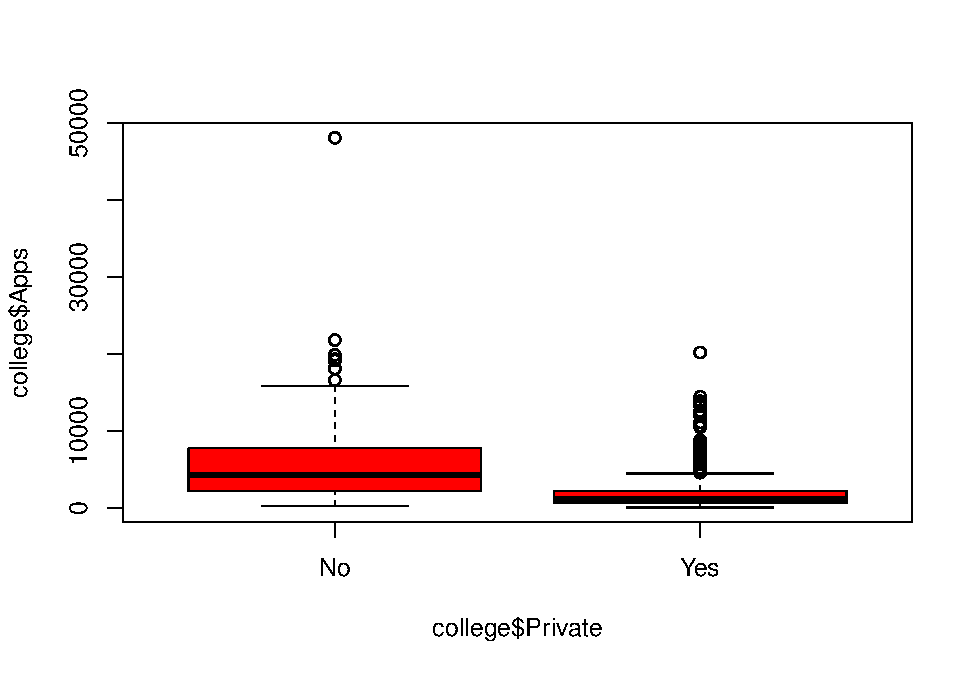
\includegraphics{assignment3_files/figure-latex/unnamed-chunk-4-1.pdf}

\hypertarget{question-4}{%
\subsubsection{Question 4}\label{question-4}}

The plot for Apps is a right tail histogram. What this shows is a large
proportion of colleges receive a small number of applications (more than
600 colleges receive less than 10000 applications). Outliers are pulling
the histogram to the right and causing larger buckets as well, further
skewing plot.

\begin{Shaded}
\begin{Highlighting}[]
\FunctionTok{hist}\NormalTok{(college}\SpecialCharTok{$}\NormalTok{Apps)}
\end{Highlighting}
\end{Shaded}

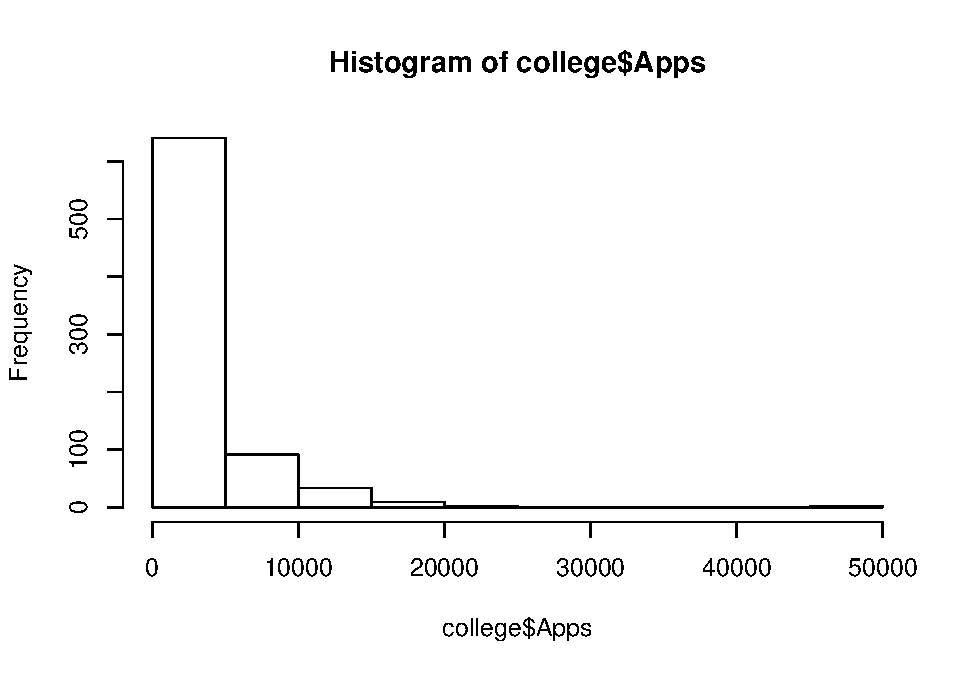
\includegraphics{assignment3_files/figure-latex/unnamed-chunk-5-1.pdf}

\hypertarget{question-5}{%
\subsubsection{Question 5}\label{question-5}}

Distribution is now corrected and more symmetric after replacing with
logarithm of Apps.

\begin{Shaded}
\begin{Highlighting}[]
\NormalTok{college}\SpecialCharTok{$}\NormalTok{Apps }\OtherTok{\textless{}{-}} \FunctionTok{log}\NormalTok{(college}\SpecialCharTok{$}\NormalTok{Apps)}
\FunctionTok{hist}\NormalTok{(college}\SpecialCharTok{$}\NormalTok{Apps)}
\end{Highlighting}
\end{Shaded}

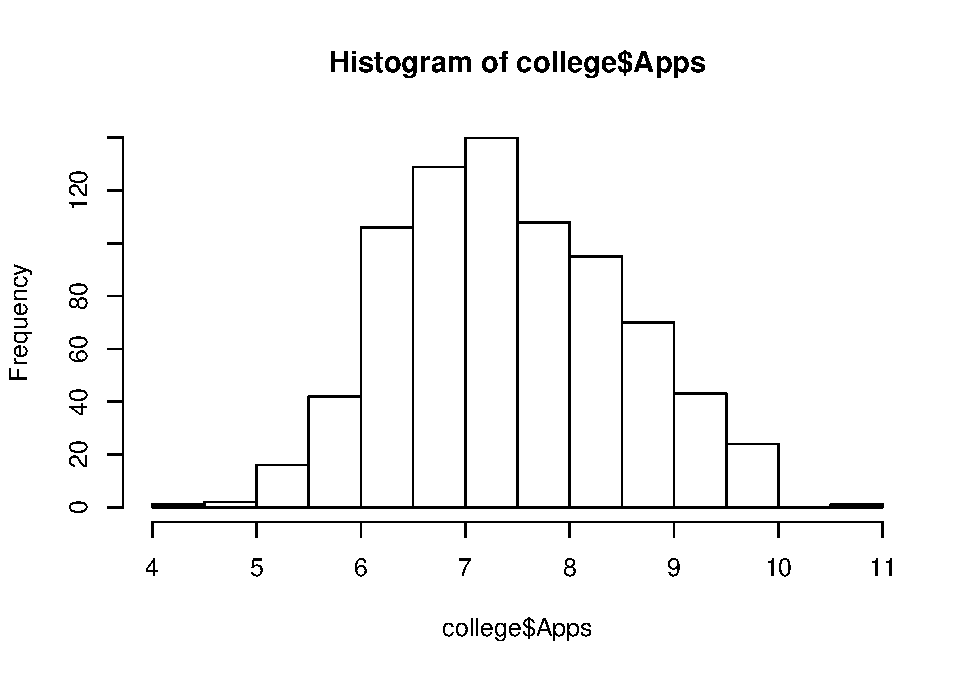
\includegraphics{assignment3_files/figure-latex/unnamed-chunk-6-1.pdf}

\hypertarget{question-6}{%
\subsubsection{Question 6}\label{question-6}}

Replaced Top10perc with Elite column

\begin{Shaded}
\begin{Highlighting}[]
\NormalTok{college}\SpecialCharTok{$}\NormalTok{Elite }\OtherTok{\textless{}{-}} \FunctionTok{as.factor}\NormalTok{(}\FunctionTok{ifelse}\NormalTok{(college}\SpecialCharTok{$}\NormalTok{Top10perc }\SpecialCharTok{\textgreater{}=} \DecValTok{50}\NormalTok{, }\StringTok{"Yes"}\NormalTok{, }\StringTok{"No"}\NormalTok{))}
\NormalTok{college}\SpecialCharTok{$}\NormalTok{Top10perc }\OtherTok{\textless{}{-}} \ConstantTok{NULL}
\end{Highlighting}
\end{Shaded}

\hypertarget{question-7}{%
\subsubsection{Question 7}\label{question-7}}

There is a statistically significant difference as shown by the
p-value\textless alpha and side by side box plot. ``Yes'' has a
statistically different mean that is higher than ``No''. Thus, it may
benefit using the new Elite feature that was based on the previously not
recommended Top10perc feature.

\begin{Shaded}
\begin{Highlighting}[]
\CommentTok{\# Categoric}
\FunctionTok{t.test}\NormalTok{(college}\SpecialCharTok{$}\NormalTok{Apps}\SpecialCharTok{\textasciitilde{}}\NormalTok{college}\SpecialCharTok{$}\NormalTok{Elite, }\AttributeTok{alternative=}\StringTok{"two.sided"}\NormalTok{)}
\end{Highlighting}
\end{Shaded}

\begin{verbatim}
## 
##  Welch Two Sample t-test
## 
## data:  college$Apps by college$Elite
## t = -8.4365, df = 106.26, p-value = 0.0000000000001778
## alternative hypothesis: true difference in means is not equal to 0
## 95 percent confidence interval:
##  -1.176238 -0.728607
## sample estimates:
##  mean in group No mean in group Yes 
##          7.324853          8.277275
\end{verbatim}

\begin{Shaded}
\begin{Highlighting}[]
\FunctionTok{plot}\NormalTok{(college}\SpecialCharTok{$}\NormalTok{Apps}\SpecialCharTok{\textasciitilde{}}\NormalTok{college}\SpecialCharTok{$}\NormalTok{Elite, }\AttributeTok{col=}\StringTok{"red"}\NormalTok{)}
\end{Highlighting}
\end{Shaded}

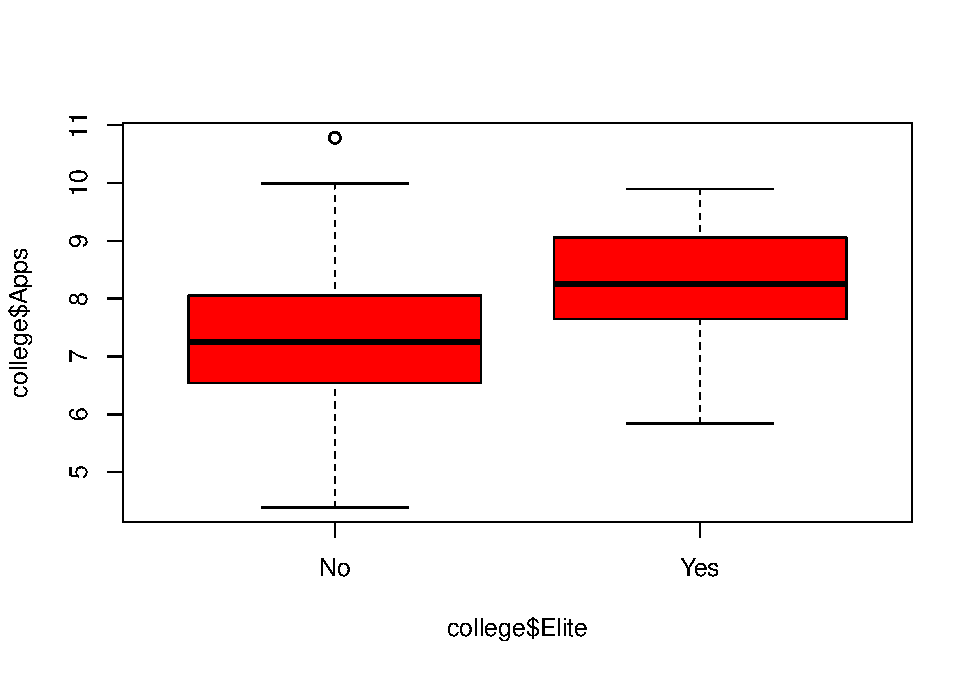
\includegraphics{assignment3_files/figure-latex/unnamed-chunk-8-1.pdf}

\hypertarget{question-8}{%
\subsubsection{Question 8}\label{question-8}}

Data split on initial run according to 80\% or apprxoimately 621
observations.

\begin{Shaded}
\begin{Highlighting}[]
\NormalTok{smp\_size }\OtherTok{\textless{}{-}} \FunctionTok{floor}\NormalTok{(.}\DecValTok{80} \SpecialCharTok{*} \FunctionTok{nrow}\NormalTok{(college))}
\NormalTok{smp\_size\_plus }\OtherTok{\textless{}{-}}\NormalTok{ smp\_size}\SpecialCharTok{+}\DecValTok{1}
\NormalTok{pop\_size }\OtherTok{\textless{}{-}} \FunctionTok{as.numeric}\NormalTok{(}\FunctionTok{nrow}\NormalTok{(college))}

\NormalTok{college\_train }\OtherTok{\textless{}{-}}\NormalTok{ college[}\DecValTok{1}\SpecialCharTok{:}\NormalTok{smp\_size,]}
\NormalTok{college\_test }\OtherTok{\textless{}{-}}\NormalTok{ college[smp\_size\_plus}\SpecialCharTok{:}\NormalTok{pop\_size,]}
\end{Highlighting}
\end{Shaded}

\hypertarget{question-9}{%
\subsubsection{Question 9}\label{question-9}}

\begin{Shaded}
\begin{Highlighting}[]
\FunctionTok{set.seed}\NormalTok{(}\DecValTok{123}\NormalTok{)}
\end{Highlighting}
\end{Shaded}

\hypertarget{question-10}{%
\subsubsection{Question 10}\label{question-10}}

Linear Regression with 10 fold cross validation with all features. The
model shows PrivateYes, Accept, Enroll, S.F.Ratio, Expend, and Grad.Rate
as all statistically different from 0. This means these variables have a
statistically significant effect on the outcome variable Apps.

\begin{Shaded}
\begin{Highlighting}[]
\FunctionTok{set.seed}\NormalTok{(}\DecValTok{123}\NormalTok{)}
\FunctionTok{attach}\NormalTok{(college)}
\NormalTok{train.control }\OtherTok{\textless{}{-}} \FunctionTok{trainControl}\NormalTok{(}\AttributeTok{method=}\StringTok{"cv"}\NormalTok{, }\AttributeTok{number=}\DecValTok{10}\NormalTok{)}
\NormalTok{college\_kf }\OtherTok{\textless{}{-}} \FunctionTok{train}\NormalTok{(Apps}\SpecialCharTok{\textasciitilde{}}\NormalTok{., }
                      \AttributeTok{data=}\NormalTok{college, }
                      \AttributeTok{method=}\StringTok{"lm"}\NormalTok{, }
                      \AttributeTok{trControl=}\NormalTok{train.control)}
\FunctionTok{print}\NormalTok{(college\_kf)}
\end{Highlighting}
\end{Shaded}

\begin{verbatim}
## Linear Regression 
## 
## 777 samples
##  17 predictor
## 
## No pre-processing
## Resampling: Cross-Validated (10 fold) 
## Summary of sample sizes: 699, 698, 699, 700, 700, 700, ... 
## Resampling results:
## 
##   RMSE       Rsquared   MAE      
##   0.5289996  0.7733852  0.4009352
## 
## Tuning parameter 'intercept' was held constant at a value of TRUE
\end{verbatim}

\begin{Shaded}
\begin{Highlighting}[]
\FunctionTok{summary}\NormalTok{(college\_kf)}
\end{Highlighting}
\end{Shaded}

\begin{verbatim}
## 
## Call:
## lm(formula = .outcome ~ ., data = dat)
## 
## Residuals:
##      Min       1Q   Median       3Q      Max 
## -2.53509 -0.28293  0.06619  0.32455  1.60151 
## 
## Coefficients:
##                 Estimate   Std. Error t value             Pr(>|t|)    
## (Intercept)  4.530590882  0.197584840  22.930 < 0.0000000000000002 ***
## PrivateYes  -0.584850786  0.068586187  -8.527 < 0.0000000000000002 ***
## Accept       0.000168406  0.000019926   8.452 < 0.0000000000000002 ***
## Enroll       0.000379716  0.000091467   4.151       0.000036788523 ***
## Top25perc    0.004433600  0.001457516   3.042              0.00243 ** 
## F.Undergrad -0.000040815  0.000016176  -2.523              0.01183 *  
## P.Undergrad  0.000036368  0.000015851   2.294              0.02204 *  
## Outstate     0.000030927  0.000009398   3.291              0.00105 ** 
## Room.Board   0.000059407  0.000023851   2.491              0.01296 *  
## Books        0.000310677  0.000117622   2.641              0.00843 ** 
## Personal     0.000046997  0.000031141   1.509              0.13167    
## PhD          0.005777735  0.002275018   2.540              0.01129 *  
## Terminal     0.001349676  0.002498401   0.540              0.58921    
## S.F.Ratio    0.040811202  0.006426354   6.351       0.000000000369 ***
## perc.alumni -0.005389642  0.002024787  -2.662              0.00794 ** 
## Expend       0.000024241  0.000005931   4.087       0.000048339640 ***
## Grad.Rate    0.007891464  0.001453742   5.428       0.000000076580 ***
## EliteYes     0.108712180  0.081922878   1.327              0.18491    
## ---
## Signif. codes:  0 '***' 0.001 '**' 0.01 '*' 0.05 '.' 0.1 ' ' 1
## 
## Residual standard error: 0.5141 on 759 degrees of freedom
## Multiple R-squared:  0.7757, Adjusted R-squared:  0.7707 
## F-statistic: 154.4 on 17 and 759 DF,  p-value: < 0.00000000000000022
\end{verbatim}

\hypertarget{question-11}{%
\subsubsection{Question 11}\label{question-11}}

\begin{Shaded}
\begin{Highlighting}[]
\FunctionTok{set.seed}\NormalTok{(}\DecValTok{123}\NormalTok{)}
\NormalTok{college\_pred }\OtherTok{\textless{}{-}} \FunctionTok{predict}\NormalTok{(college\_kf, college\_test)}
\NormalTok{RMSE }\OtherTok{\textless{}{-}} \FunctionTok{sqrt}\NormalTok{(}\FunctionTok{mean}\NormalTok{(}\FunctionTok{abs}\NormalTok{(college\_test}\SpecialCharTok{$}\NormalTok{Apps}\SpecialCharTok{{-}}\NormalTok{college\_pred)}\SpecialCharTok{\^{}}\DecValTok{2}\NormalTok{))}
\NormalTok{RMSE}
\end{Highlighting}
\end{Shaded}

\begin{verbatim}
## [1] 0.4650652
\end{verbatim}

\hypertarget{question-12}{%
\subsubsection{Question 12}\label{question-12}}

\begin{Shaded}
\begin{Highlighting}[]
\FunctionTok{set.seed}\NormalTok{(}\DecValTok{123}\NormalTok{)}
\end{Highlighting}
\end{Shaded}

\hypertarget{question-13}{%
\subsubsection{Question 13}\label{question-13}}

nvmax=13 has the lowest cross validation RMSE of .5477043. Variables
selected were PrivateYes, Accept, Enroll, Top25perc, F.Undergrad,
Outstate, Room.Board, Books, PhD, S.F.Ratio, perc.alumni, Expend, and
Grad.Rate.

\begin{Shaded}
\begin{Highlighting}[]
\FunctionTok{set.seed}\NormalTok{(}\DecValTok{123}\NormalTok{)}
\NormalTok{train.control }\OtherTok{\textless{}{-}} \FunctionTok{trainControl}\NormalTok{(}\AttributeTok{method=}\StringTok{"cv"}\NormalTok{, }\AttributeTok{number=}\DecValTok{10}\NormalTok{)}
\NormalTok{college\_stepBk }\OtherTok{\textless{}{-}} \FunctionTok{train}\NormalTok{(Apps}\SpecialCharTok{\textasciitilde{}}\NormalTok{.,}
                        \AttributeTok{data=}\NormalTok{college\_train,}
                        \AttributeTok{method=}\StringTok{"leapBackward"}\NormalTok{,}
                        \AttributeTok{trControl=}\NormalTok{train.control,}
                        \AttributeTok{tuneGrid=}\FunctionTok{data.frame}\NormalTok{(}\AttributeTok{nvmax=}\DecValTok{1}\SpecialCharTok{:}\DecValTok{16}\NormalTok{))}
\CommentTok{\#print(college\_stepBk)}
\FunctionTok{summary}\NormalTok{(college\_stepBk}\SpecialCharTok{$}\NormalTok{finalModel)}
\end{Highlighting}
\end{Shaded}

\begin{verbatim}
## Subset selection object
## 17 Variables  (and intercept)
##             Forced in Forced out
## PrivateYes      FALSE      FALSE
## Accept          FALSE      FALSE
## Enroll          FALSE      FALSE
## Top25perc       FALSE      FALSE
## F.Undergrad     FALSE      FALSE
## P.Undergrad     FALSE      FALSE
## Outstate        FALSE      FALSE
## Room.Board      FALSE      FALSE
## Books           FALSE      FALSE
## Personal        FALSE      FALSE
## PhD             FALSE      FALSE
## Terminal        FALSE      FALSE
## S.F.Ratio       FALSE      FALSE
## perc.alumni     FALSE      FALSE
## Expend          FALSE      FALSE
## Grad.Rate       FALSE      FALSE
## EliteYes        FALSE      FALSE
## 1 subsets of each size up to 13
## Selection Algorithm: backward
##           PrivateYes Accept Enroll Top25perc F.Undergrad P.Undergrad Outstate
## 1  ( 1 )  " "        "*"    " "    " "       " "         " "         " "     
## 2  ( 1 )  " "        "*"    " "    "*"       " "         " "         " "     
## 3  ( 1 )  "*"        "*"    " "    "*"       " "         " "         " "     
## 4  ( 1 )  "*"        "*"    " "    "*"       " "         " "         " "     
## 5  ( 1 )  "*"        "*"    " "    "*"       " "         " "         " "     
## 6  ( 1 )  "*"        "*"    " "    "*"       " "         " "         " "     
## 7  ( 1 )  "*"        "*"    " "    "*"       " "         " "         "*"     
## 8  ( 1 )  "*"        "*"    "*"    "*"       " "         " "         "*"     
## 9  ( 1 )  "*"        "*"    "*"    "*"       " "         " "         "*"     
## 10  ( 1 ) "*"        "*"    "*"    "*"       " "         " "         "*"     
## 11  ( 1 ) "*"        "*"    "*"    "*"       " "         " "         "*"     
## 12  ( 1 ) "*"        "*"    "*"    "*"       "*"         " "         "*"     
## 13  ( 1 ) "*"        "*"    "*"    "*"       "*"         " "         "*"     
##           Room.Board Books Personal PhD Terminal S.F.Ratio perc.alumni Expend
## 1  ( 1 )  " "        " "   " "      " " " "      " "       " "         " "   
## 2  ( 1 )  " "        " "   " "      " " " "      " "       " "         " "   
## 3  ( 1 )  " "        " "   " "      " " " "      " "       " "         " "   
## 4  ( 1 )  " "        " "   " "      " " " "      " "       " "         " "   
## 5  ( 1 )  " "        " "   " "      " " " "      " "       " "         "*"   
## 6  ( 1 )  " "        " "   " "      " " " "      "*"       " "         "*"   
## 7  ( 1 )  " "        " "   " "      " " " "      "*"       " "         "*"   
## 8  ( 1 )  " "        " "   " "      " " " "      "*"       " "         "*"   
## 9  ( 1 )  " "        " "   " "      "*" " "      "*"       " "         "*"   
## 10  ( 1 ) " "        " "   " "      "*" " "      "*"       "*"         "*"   
## 11  ( 1 ) " "        "*"   " "      "*" " "      "*"       "*"         "*"   
## 12  ( 1 ) " "        "*"   " "      "*" " "      "*"       "*"         "*"   
## 13  ( 1 ) "*"        "*"   " "      "*" " "      "*"       "*"         "*"   
##           Grad.Rate EliteYes
## 1  ( 1 )  " "       " "     
## 2  ( 1 )  " "       " "     
## 3  ( 1 )  " "       " "     
## 4  ( 1 )  "*"       " "     
## 5  ( 1 )  "*"       " "     
## 6  ( 1 )  "*"       " "     
## 7  ( 1 )  "*"       " "     
## 8  ( 1 )  "*"       " "     
## 9  ( 1 )  "*"       " "     
## 10  ( 1 ) "*"       " "     
## 11  ( 1 ) "*"       " "     
## 12  ( 1 ) "*"       " "     
## 13  ( 1 ) "*"       " "
\end{verbatim}

\hypertarget{question-14}{%
\subsubsection{Question 14}\label{question-14}}

RMSE was \textasciitilde.489 for the Stepwise Backward function.

\begin{Shaded}
\begin{Highlighting}[]
\NormalTok{college\_stepBk\_pred }\OtherTok{\textless{}{-}} \FunctionTok{predict}\NormalTok{(college\_stepBk, college\_test)}
\NormalTok{RMSE\_stepBk }\OtherTok{\textless{}{-}} \FunctionTok{sqrt}\NormalTok{(}\FunctionTok{mean}\NormalTok{(}\FunctionTok{abs}\NormalTok{(college\_test}\SpecialCharTok{$}\NormalTok{Apps}\SpecialCharTok{{-}}\NormalTok{college\_stepBk\_pred)}\SpecialCharTok{\^{}}\DecValTok{2}\NormalTok{))}
\NormalTok{RMSE\_stepBk}
\end{Highlighting}
\end{Shaded}

\begin{verbatim}
## [1] 0.4889923
\end{verbatim}

\hypertarget{question-15}{%
\subsubsection{Question 15}\label{question-15}}

\begin{Shaded}
\begin{Highlighting}[]
\NormalTok{college\_rpart }\OtherTok{\textless{}{-}} \FunctionTok{rpart}\NormalTok{(Apps}\SpecialCharTok{\textasciitilde{}}\NormalTok{., }\AttributeTok{data=}\NormalTok{college\_train)}
\NormalTok{college\_rpart\_pred }\OtherTok{\textless{}{-}} \FunctionTok{predict}\NormalTok{(college\_rpart, college\_test)}

\NormalTok{RMSE\_rpart }\OtherTok{\textless{}{-}} \FunctionTok{sqrt}\NormalTok{(}\FunctionTok{mean}\NormalTok{(}\FunctionTok{abs}\NormalTok{(college\_test}\SpecialCharTok{$}\NormalTok{Apps}\SpecialCharTok{{-}}\NormalTok{college\_rpart\_pred)}\SpecialCharTok{\^{}}\DecValTok{2}\NormalTok{))}
\NormalTok{RMSE\_rpart}
\end{Highlighting}
\end{Shaded}

\begin{verbatim}
## [1] 0.2985149
\end{verbatim}

\hypertarget{question-16}{%
\subsubsection{Question 16}\label{question-16}}

The RMSE for Linear Regression, Stepwise Regression, and the Regression
Tree is .529, .489, and .299, respectively. This indicates the
Regression Tree model has a better error rate, although this may need to
be tested against new data.

\hypertarget{problem-2}{%
\subsection{Problem 2}\label{problem-2}}

\hypertarget{question-1-1}{%
\subsubsection{Question 1}\label{question-1-1}}

Read in data, no observed nulls or zero values. Create train and test
set.

\begin{Shaded}
\begin{Highlighting}[]
\FunctionTok{set.seed}\NormalTok{(}\DecValTok{123}\NormalTok{)}
\NormalTok{credit }\OtherTok{\textless{}{-}} \FunctionTok{read.csv}\NormalTok{(}\StringTok{"data/credit.csv"}\NormalTok{, }\AttributeTok{stringsAsFactors=}\ConstantTok{TRUE}\NormalTok{)}
\CommentTok{\# Summary of data}
\FunctionTok{summary}\NormalTok{(credit)}
\end{Highlighting}
\end{Shaded}

\begin{verbatim}
##    checking_balance months_loan_duration   credit_history
##  < 0 DM    :274     Min.   : 4.0         critical :293   
##  > 200 DM  : 63     1st Qu.:12.0         good     :530   
##  1 - 200 DM:269     Median :18.0         perfect  : 40   
##  unknown   :394     Mean   :20.9         poor     : 88   
##                     3rd Qu.:24.0         very good: 49   
##                     Max.   :72.0                         
##                  purpose        amount           savings_balance
##  business            : 97   Min.   :  250   < 100 DM     :603   
##  car                 :337   1st Qu.: 1366   > 1000 DM    : 48   
##  car0                : 12   Median : 2320   100 - 500 DM :103   
##  education           : 59   Mean   : 3271   500 - 1000 DM: 63   
##  furniture/appliances:473   3rd Qu.: 3972   unknown      :183   
##  renovations         : 22   Max.   :18424                       
##   employment_duration percent_of_income years_at_residence      age       
##  < 1 year   :172      Min.   :1.000     Min.   :1.000      Min.   :19.00  
##  > 7 years  :253      1st Qu.:2.000     1st Qu.:2.000      1st Qu.:27.00  
##  1 - 4 years:339      Median :3.000     Median :3.000      Median :33.00  
##  4 - 7 years:174      Mean   :2.973     Mean   :2.845      Mean   :35.55  
##  unemployed : 62      3rd Qu.:4.000     3rd Qu.:4.000      3rd Qu.:42.00  
##                       Max.   :4.000     Max.   :4.000      Max.   :75.00  
##  other_credit  housing    existing_loans_count         job        dependents   
##  bank :139    other:108   Min.   :1.000        management:148   Min.   :1.000  
##  none :814    own  :713   1st Qu.:1.000        skilled   :630   1st Qu.:1.000  
##  store: 47    rent :179   Median :1.000        unemployed: 22   Median :1.000  
##                           Mean   :1.407        unskilled :200   Mean   :1.155  
##                           3rd Qu.:2.000                         3rd Qu.:1.000  
##                           Max.   :4.000                         Max.   :2.000  
##  phone     default  
##  no :596   no :700  
##  yes:404   yes:300  
##                     
##                     
##                     
## 
\end{verbatim}

\begin{Shaded}
\begin{Highlighting}[]
\CommentTok{\# View Null and NA}
\FunctionTok{colSums}\NormalTok{(credit }\SpecialCharTok{==} \DecValTok{0} \SpecialCharTok{|} \FunctionTok{is.na}\NormalTok{(credit))}
\end{Highlighting}
\end{Shaded}

\begin{verbatim}
##     checking_balance months_loan_duration       credit_history 
##                    0                    0                    0 
##              purpose               amount      savings_balance 
##                    0                    0                    0 
##  employment_duration    percent_of_income   years_at_residence 
##                    0                    0                    0 
##                  age         other_credit              housing 
##                    0                    0                    0 
## existing_loans_count                  job           dependents 
##                    0                    0                    0 
##                phone              default 
##                    0                    0
\end{verbatim}

\begin{Shaded}
\begin{Highlighting}[]
\CommentTok{\# split train and test set}
\NormalTok{train\_sample }\OtherTok{\textless{}{-}} \FunctionTok{sample}\NormalTok{(}\DecValTok{1000}\NormalTok{, }\DecValTok{900}\NormalTok{)}
\NormalTok{credit\_train }\OtherTok{\textless{}{-}}\NormalTok{ credit[train\_sample,]}
\NormalTok{credit\_test }\OtherTok{\textless{}{-}}\NormalTok{ credit[}\SpecialCharTok{{-}}\NormalTok{train\_sample,]}
\end{Highlighting}
\end{Shaded}

\hypertarget{question-2-1}{%
\subsubsection{Question 2}\label{question-2-1}}

Train using glm to predict default on test

\begin{Shaded}
\begin{Highlighting}[]
\FunctionTok{library}\NormalTok{(gmodels)}
\end{Highlighting}
\end{Shaded}

\begin{verbatim}
## Warning: package 'gmodels' was built under R version 3.6.3
\end{verbatim}

\begin{Shaded}
\begin{Highlighting}[]
\FunctionTok{set.seed}\NormalTok{(}\DecValTok{123}\NormalTok{)}
\NormalTok{credit\_glm }\OtherTok{\textless{}{-}} \FunctionTok{glm}\NormalTok{(credit\_train}\SpecialCharTok{$}\NormalTok{default}\SpecialCharTok{\textasciitilde{}}\NormalTok{., }\AttributeTok{data=}\NormalTok{credit\_train, }\AttributeTok{family=}\StringTok{"binomial"}\NormalTok{)}
\NormalTok{credit\_pred }\OtherTok{\textless{}{-}} \FunctionTok{predict}\NormalTok{(credit\_glm, credit\_test, }\AttributeTok{type=}\StringTok{"response"}\NormalTok{)}
\NormalTok{credit\_pred\_label }\OtherTok{\textless{}{-}} \FunctionTok{as.factor}\NormalTok{(}\FunctionTok{ifelse}\NormalTok{(credit\_pred}\SpecialCharTok{\textgreater{}}\NormalTok{.}\DecValTok{5}\NormalTok{, }\StringTok{"yes"}\NormalTok{, }\StringTok{"no"}\NormalTok{))}
\end{Highlighting}
\end{Shaded}

\hypertarget{question-3-1}{%
\subsubsection{Question 3}\label{question-3-1}}

7 out of 65 no default were categorized as yes default by the model,
this is a FPR of \textasciitilde13\%. The model is a \textasciitilde8\%
worse to the C5 after improvement but better some other methods tested
based on the FPR.

\begin{Shaded}
\begin{Highlighting}[]
\NormalTok{t}\OtherTok{=}\FunctionTok{table}\NormalTok{(credit\_test}\SpecialCharTok{$}\NormalTok{default, credit\_pred\_label)}
\NormalTok{FPR}\OtherTok{=}\NormalTok{t[}\DecValTok{1}\NormalTok{,}\DecValTok{2}\NormalTok{]}\SpecialCharTok{/}\NormalTok{(t[}\DecValTok{1}\NormalTok{,}\DecValTok{2}\NormalTok{]}\SpecialCharTok{+}\NormalTok{t[}\DecValTok{1}\NormalTok{,}\DecValTok{1}\NormalTok{])}
\NormalTok{FPR}
\end{Highlighting}
\end{Shaded}

\begin{verbatim}
## [1] 0.1076923
\end{verbatim}

\begin{Shaded}
\begin{Highlighting}[]
\FunctionTok{CrossTable}\NormalTok{(credit\_pred\_label, credit\_test}\SpecialCharTok{$}\NormalTok{default, }
           \AttributeTok{prop.chisq=}\ConstantTok{FALSE}\NormalTok{, }
           \AttributeTok{prop.t=}\ConstantTok{FALSE}\NormalTok{,}
           \AttributeTok{dnn=}\FunctionTok{c}\NormalTok{(}\StringTok{"predicted"}\NormalTok{,}\StringTok{"actual"}\NormalTok{))}
\end{Highlighting}
\end{Shaded}

\begin{verbatim}
## 
##  
##    Cell Contents
## |-------------------------|
## |                       N |
## |           N / Row Total |
## |           N / Col Total |
## |-------------------------|
## 
##  
## Total Observations in Table:  100 
## 
##  
##              | actual 
##    predicted |        no |       yes | Row Total | 
## -------------|-----------|-----------|-----------|
##           no |        58 |        19 |        77 | 
##              |     0.753 |     0.247 |     0.770 | 
##              |     0.892 |     0.543 |           | 
## -------------|-----------|-----------|-----------|
##          yes |         7 |        16 |        23 | 
##              |     0.304 |     0.696 |     0.230 | 
##              |     0.108 |     0.457 |           | 
## -------------|-----------|-----------|-----------|
## Column Total |        65 |        35 |       100 | 
##              |     0.650 |     0.350 |           | 
## -------------|-----------|-----------|-----------|
## 
## 
\end{verbatim}

\hypertarget{question-4-1}{%
\subsubsection{Question 4}\label{question-4-1}}

FPR was \textasciitilde29.9\% and FNR \textasciitilde20.3\%, so this
method is worse for FPR and better for FNR. This is quite interesting as
there are more Yes values now in the training set. In the case of this
dataset it may be better to not change the sampling because it is only a
70/30 split for No/Yes. If the original dataset was closer to 90/10 or
95/5 it may have shown an improvement over original models.

\begin{Shaded}
\begin{Highlighting}[]
\FunctionTok{set.seed}\NormalTok{(}\DecValTok{123}\NormalTok{)}
\FunctionTok{library}\NormalTok{(DMwR)}
\end{Highlighting}
\end{Shaded}

\begin{verbatim}
## Warning: package 'DMwR' was built under R version 3.6.3
\end{verbatim}

\begin{verbatim}
## Loading required package: grid
\end{verbatim}

\begin{verbatim}
## Registered S3 method overwritten by 'quantmod':
##   method            from
##   as.zoo.data.frame zoo
\end{verbatim}

\begin{Shaded}
\begin{Highlighting}[]
\CommentTok{\# Over sample using SMOTE}
\NormalTok{credit\_smote }\OtherTok{\textless{}{-}} \FunctionTok{SMOTE}\NormalTok{(default}\SpecialCharTok{\textasciitilde{}}\NormalTok{., }\AttributeTok{data=}\NormalTok{credit\_train, }\AttributeTok{perc.over=}\DecValTok{100}\NormalTok{)}
\CommentTok{\# Train new model}
\NormalTok{credit\_smote\_glm }\OtherTok{\textless{}{-}} \FunctionTok{glm}\NormalTok{(credit\_smote}\SpecialCharTok{$}\NormalTok{default}\SpecialCharTok{\textasciitilde{}}\NormalTok{., }\AttributeTok{data=}\NormalTok{credit\_smote, }\AttributeTok{family=}\StringTok{"binomial"}\NormalTok{)}
\NormalTok{credit\_smote\_pred }\OtherTok{\textless{}{-}} \FunctionTok{predict}\NormalTok{(credit\_smote\_glm, credit\_test, }\AttributeTok{type=}\StringTok{"response"}\NormalTok{)}
\NormalTok{credit\_smote\_pred\_label }\OtherTok{\textless{}{-}} \FunctionTok{as.factor}\NormalTok{(}\FunctionTok{ifelse}\NormalTok{(credit\_smote\_pred}\SpecialCharTok{\textgreater{}}\NormalTok{.}\DecValTok{5}\NormalTok{, }\StringTok{"yes"}\NormalTok{, }\StringTok{"no"}\NormalTok{))}
\CommentTok{\# View FPR/FNR and error rate}
\NormalTok{t}\OtherTok{=}\FunctionTok{table}\NormalTok{(credit\_test}\SpecialCharTok{$}\NormalTok{default, credit\_smote\_pred\_label)}
\NormalTok{FPR}\OtherTok{=}\NormalTok{t[}\DecValTok{1}\NormalTok{,}\DecValTok{2}\NormalTok{]}\SpecialCharTok{/}\NormalTok{(t[}\DecValTok{1}\NormalTok{,}\DecValTok{2}\NormalTok{]}\SpecialCharTok{+}\NormalTok{t[}\DecValTok{1}\NormalTok{,}\DecValTok{1}\NormalTok{])}
\NormalTok{FPR}
\end{Highlighting}
\end{Shaded}

\begin{verbatim}
## [1] 0.2461538
\end{verbatim}

\begin{Shaded}
\begin{Highlighting}[]
\FunctionTok{CrossTable}\NormalTok{(credit\_smote\_pred\_label, credit\_test}\SpecialCharTok{$}\NormalTok{default, }
           \AttributeTok{prop.chisq=}\ConstantTok{FALSE}\NormalTok{, }
           \AttributeTok{prop.t=}\ConstantTok{FALSE}\NormalTok{,}
           \AttributeTok{dnn=}\FunctionTok{c}\NormalTok{(}\StringTok{"predicted"}\NormalTok{,}\StringTok{"actual"}\NormalTok{))}
\end{Highlighting}
\end{Shaded}

\begin{verbatim}
## 
##  
##    Cell Contents
## |-------------------------|
## |                       N |
## |           N / Row Total |
## |           N / Col Total |
## |-------------------------|
## 
##  
## Total Observations in Table:  100 
## 
##  
##              | actual 
##    predicted |        no |       yes | Row Total | 
## -------------|-----------|-----------|-----------|
##           no |        49 |        12 |        61 | 
##              |     0.803 |     0.197 |     0.610 | 
##              |     0.754 |     0.343 |           | 
## -------------|-----------|-----------|-----------|
##          yes |        16 |        23 |        39 | 
##              |     0.410 |     0.590 |     0.390 | 
##              |     0.246 |     0.657 |           | 
## -------------|-----------|-----------|-----------|
## Column Total |        65 |        35 |       100 | 
##              |     0.650 |     0.350 |           | 
## -------------|-----------|-----------|-----------|
## 
## 
\end{verbatim}


\end{document}
